% !TeX spellcheck = en_US
\documentclass[letterpaper,12pt,twoside]{report}
\usepackage{fancyhdr}
\usepackage{fullpage}
\usepackage{tikz}
\usepackage{amsmath}

\begin{document}
	\pagestyle{fancy}
	\fancyhf{}
	\fancyhead[L]{Day 3}
	\fancyhead[R]{\textit{The Calendar Project}}
	\fancyfoot[L]{Citations Involved: none}
	
	% Problem
	\paragraph{Problem}
	\begin{quote}
	\textsf{When all the diagonals in a regular hexagon are drawn, how many pairs of diagonals will be perpendicular?}
	\end{quote}
	
	% Graphics
	\begin{center}
		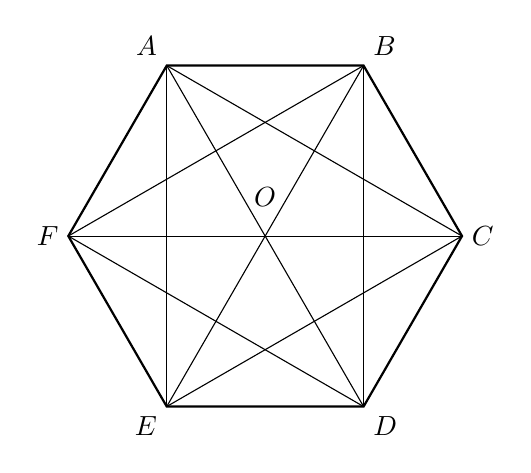
\begin{tikzpicture}[scale=0.5]
		\draw[thick] (5,0) -- (2.5,-4.33) -- (-2.5,-4.33) -- (-5,0) -- (-2.5,4.33) -- (2.5,4.33) -- cycle;
		\draw (5,0) -- (-2.5,4.33);
		\draw (5,0) -- (-5,0);
		\draw (5,0) -- (-2.5,-4.33);
		\draw (-5,0) -- (2.5,4.33);
		\draw (-5,0) -- (2.5,-4.33);
		\draw (-2.5,4.33) -- (-2.5,-4.33);
		\draw (-2.5,4.33) -- (2.5,-4.33);
		\draw (2.5,4.33) -- (-2.5,-4.33);
		\draw (2.5,4.33) -- (2.5,-4.33);
		
		\node[above left] at (-2.5,4.33) {$A$};
		\node[above right] at (2.5,4.33) {$B$};
		\node[right] at (5,0) {$C$};
		\node[below right] at (2.5,-4.33) {$D$};
		\node[below left] at (-2.5,-4.33) {$E$};
		\node[left] at (-5,0) {$F$};
		\node[above] at (0,0.5) {$O$};
		
		\end{tikzpicture}
	\end{center}
	
	% Reasoning
	\paragraph{Reasoning}
	\begin{quotation}
	
	Given that the hexagon is regular, it is equilateral and equiangular by definition (1); therefore $\overline{AB}\cong\overline{BC}\cong\overline{CD}\cong\overline{DE}\cong\overline{EF}\cong\overline{FA}$ and $\angle FAB\cong\angle ABC\cong\angle BCD\cong\angle CDE\cong\angle DEF\cong\angle EFA$. Thus $\triangle FAB\cong\triangle ABC\cong\triangle BCD\cong\triangle CDE\cong\triangle DEF\cong\triangle EFA$ by SAS. The definition of a kite is ``a quadrilateral with exactly two pairs of congruent consecutive sides'' (2). With $\overline{AF}\cong\overline{FE}$ and $\overline{AC}\cong\overline{CE}$ by CPCTC, quadrilateral $AFEC$ is a kite by definition (2); with $\overline{BC}\cong\overline{CD}$ and $\overline{BF}\cong\overline{FD}$ by CPCTC, quadrilateral $BCDF$ is a kite by definition (2); with $\overline{BA}\cong\overline{AF}$ and $\overline{BD}\cong\overline{DF}$ by CPCTC, quadrilateral $BAFD$ is a kite by definition (2); with $\overline{CD}\cong\overline{DE}$ and $\overline{CA}\cong\overline{AE}$ by CPCTC, quadrilateral $CDEA$ is a kite by definition (2); with $\overline{AB}\cong\overline{BC}$ and $\overline{AE}\cong\overline{EC}$ by CPCTC, quadrilateral $ABCE$ is a kite by definition (2); with $\overline{FE}\cong\overline{ED}$ and $\overline{FB}\cong\overline{BD}$ by CPCTC, quadrilateral $FEDB$ is a kite by definition (2). Since the diagonals of a kite are perpendicular (3), $\overline{AE}\bot\overline{FC}$, $\overline{BD}\bot\overline{CF}$, $\overline{BF}\bot\overline{AD}$, $\overline{CE}\bot\overline{DA}$, $\overline{AC}\bot\overline{BE}$, $\overline{FD}\bot\overline{EB}$. $\boxed{6}$ perpendicular pairs of diagonals are listed.
	
	\end{quotation}
	
	\paragraph{External References}
	
	\begin{enumerate}
		\item Textbook Ch. 6, Pg. 382: Definition of a Regular Polygon
		\item Textbook Ch. 6, Pg. 427: Definition of a Kite
		\item Textbook Ch. 6, Pg. 427: Properties of Kites
	\end{enumerate}

\end{document}